\section{Geometry of fixed-block lattice epigraphs}\label{sec:movement}
An adjacent edge preserves some integer quadratic constraint at both endpoints. This shared constraint controls movement even when the edge is far from the origin. For $H=(1)$, for example, the matrices with $(b,c)=(-1/2,1)$ and $(-3/2,3)$ are adjacent: they preserve the active vectors $(1,0)$ and $(1,1)$, and the second endpoint gains $(2,1)$. Both forms are integer changes of $u^2-uy+y^2$, whose integer minimum is one; their shared equalities define a line, and the remaining inequalities stop it at these endpoints. Figure~\ref{fig:edge} shows the edge in \eqref{eq:epigraph}.

\begin{figure}[htbp]
\centering
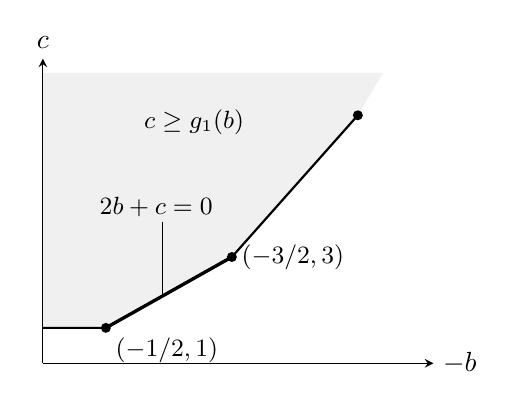
\begin{tikzpicture}[x=1.6cm,y=0.45cm,>=stealth]
\fill[gray!12] (0,1)--(0.5,1)--(1.5,3)--(2.5,7)--(2.7,8.2)--(0,8.2)--cycle;
\draw[->] (0,0)--(3.1,0) node[right] {$-b$};
\draw[->] (0,0)--(0,8.6) node[above] {$c$};
\draw[thick] (0,1)--(0.5,1)--(1.5,3)--(2.5,7);
\draw[very thick] (0.5,1)--(1.5,3);
\fill (0.5,1) circle (1.8pt) node[below right] {\small $(-1/2,1)$};
\fill (1.5,3) circle (1.8pt) node[right] {\small $(-3/2,3)$};
\fill (2.5,7) circle (1.8pt);
\node at (1.2,6.8) {\small $c\ge g_1(b)$};
\node at (0.9,4.4) {\small $2b+c=0$};
\draw[thin] (0.95,4.0)--(0.95,1.9);
\end{tikzpicture}
\caption{An explanatory slice with $H=(1)$, not a hard input from Theorem~\ref{thm:amplification}. Labels give $(b,c)$; the horizontal axis is $-b$. The highlighted edge preserves the constraint $2b+c=0$.}
\label{fig:edge}
\end{figure}

For general $H\succ0$, the defining inequalities are
$H[u]+2yb\T u+cy^2\ge1$ for $u\in\Z_+^r$ and $y\ge1$ integral. The epigraph \eqref{eq:epigraph} is their intersection. The first bound concerns the cross column $b$, not every entry of the block matrix.

\begin{theorem}[Movement along a bounded edge]\label{thm:movement}
If $(b,c)$ and $(b',c')$ are the endpoints of a bounded edge of $\mathcal E_H$, then
\begin{equation}\label{eq:movement}
 |b_i'-b_i|\le\frac12+2\sqrt{H_{ii}}\qquad(1\le i\le r).
\end{equation}
For $H=T_r$, this gives $\norm{b'-b}_\infty\le5/2$, independently of the location and order.
\end{theorem}

We compare each endpoint with a continuous quadratic minimum. The comparison first bounds the last coordinate of every active integer vector, then leaves a common term that cancels across an edge.
\subsection{Comparison with the continuous minimum}
Let $z=z(b)$ be the unique minimizer of
$x\trans Hx+2b\trans x$ over $x\ge0$, and put $\ell=b+Hz$.
Positive definiteness gives existence and uniqueness. The optimality conditions are
\begin{equation}\label{eq:kkt}
 z\ge0,\qquad \ell\ge0,\qquad z_i\ell_i=0\quad(1\le i\le r).
\end{equation}
Thus the continuous minimum is $-z\trans Hz$. We choose a fixed approximation scale to compare the discrete constraints uniformly with this minimum. The constants below will measure a positive gap and bound the last coordinate of active integer vectors. Choose an integer $q\ge2$ such that $\norm H_2r/q^2\le1/2$, where $\norm H_2$ is the spectral norm, and set
\begin{equation}\label{eq:gapconstants}
 \kappa=\frac1{2q^{2r}},\qquad Y=2q^r.
\end{equation}

\begin{lemma}[A positive gap and bounded active vectors]\label{lem:gap}
For every $b\in\R^r$,
\begin{equation}\label{eq:gap}
 z\trans Hz+\kappa\le g_H(b)\le z\trans Hz+1.
\end{equation}
The supremum in \eqref{eq:epigraph} is attained. Every active pair $(u,y)$ at $(b,g_H(b))$ satisfies, with $e=u-yz$,
\begin{equation}\label{eq:active}
 y\le Y,\qquad
 e\trans He+2y\ell\trans u
   =1-y^2\bigl(g_H(b)-z\trans Hz\bigr)\le1.
\end{equation}
The epigraph is locally polyhedral. At every vertex, $0\le\ell_i\le1/2$ for each $i$.
\end{lemma}
\begin{proof}
The comparison is based on the identity
\begin{equation}\label{eq:complete}
 \frac{1-u\trans Hu-2yb\trans u}{y^2}
 =z\trans Hz+\frac{1-e\trans He-2y\ell\trans u}{y^2}.
\end{equation}
To obtain it, substitute $b=\ell-Hz$ and use $\ell\trans z=0$. Both terms subtracted from $1$ on the right are nonnegative. Since $y\ge1$, this proves the upper bound in \eqref{eq:gap}.

For the lower bound we need one integer pair close to the continuous minimizer after scaling. Let $S=\{i:z_i>0\}$ and $s=|S|$, and let $z_S$ be the restriction of $z$ to $S$. If $s=0$, the pair $u=0,y=1$ gives the assertion. Otherwise place the $q^s+1$ coordinatewise fractional-part vectors
\[
 \{kz_S\},\qquad 0\le k\le q^s,
\]
in $q^s$ half-open boxes of side $1/q$. Two lie in the same box. Subtracting them gives $1\le y\le q^s\le q^r$ and integers $u_i$ such that $|u_i-yz_i|\le1/q$ on $S$. Put $u_i=0$ outside $S$. These integers are nonnegative: a negative integer would have distance at least one from the nonnegative number $yz_i$. Complementarity gives $\ell\trans u=0$, and
\[
 (u-yz)\trans H(u-yz)\le\norm H_2\frac r{q^2}\le\frac12.
\]
The last fraction in \eqref{eq:complete} is therefore at least $1/(2q^{2r})$. This proves the lower bound using the elementary simultaneous approximation argument, without any restriction on rationality of $b$ or $z$.

If $y>Y$, the right side of \eqref{eq:complete} is at most
$z\trans Hz+1/y^2<z\trans Hz+\kappa$.
For the finitely many remaining $y$, any value at least $z\trans Hz+\kappa$ requires $(u-yz)\trans H(u-yz)\le1$. A bounded ellipsoid contains only finitely many integer vectors. Thus the supremum is attained; multiplying \eqref{eq:complete} by $y^2$ proves \eqref{eq:active}.

These are local finiteness bounds as well. The minimizer $z(b)$ is continuous; this follows from the variational inequalities and strong convexity, which give
$\norm{z(b)-z(b')}_2\le\norm{b-b'}_2/\lambda_{\min}(H)$.
On a small neighborhood, $z$ stays bounded. All constraints that can attain the supremum there have $y\le Y$ and $(u-yz)\trans H(u-yz)\le1$, hence come from one finite list. This proves local polyhedrality.

Finally, a vertex must lie on the graph of $g_H$. Its active affine normals $(2u/y,1)$ span $\R^{r+1}$. For each $i$ at least one active $u$ has $u_i\ge1$, since otherwise their $i$th components would all vanish. Equation~\eqref{eq:active} then gives
$2y\ell_i u_i\le1$, and hence $\ell_i\le1/2$.
\end{proof}

\begin{proof}[Proof of Theorem~\ref{thm:movement}]
The epigraph is full dimensional and locally polyhedral. A bounded edge has a common active constraint $(u,y)$ at its endpoints: the equalities defining its relative interior remain equalities at both ends. At the first endpoint,
\begin{equation}\label{eq:shared}
 b+H(u/y)=\ell+He/y.
\end{equation}
Cauchy--Schwarz for the inner product defined by $H$ gives
\[
 |(He)_i|^2\le H_{ii}\,e\trans He\le H_{ii}.
\]
Together with $0\le\ell_i\le1/2$, this puts the $i$th coordinate of \eqref{eq:shared} in the interval
\[
 \left[-\frac{\sqrt{H_{ii}}}{y},\,
       \frac12+\frac{\sqrt{H_{ii}}}{y}\right].
\]
The second endpoint has the same $u$ and $y$, so subtracting cancels the term $H(u/y)$. The interval length is at most $1/2+2\sqrt{H_{ii}}$, proving \eqref{eq:movement}. Neither simplicity of a vertex nor $y=1$ has been assumed.
\end{proof}



\subsection{Integer shears and finite configurations}
The active vectors can grow with the location of a vertex. Subtracting the integer part of the continuous minimizer removes that growth. Choose an integer $t_H\ge1$ with
\begin{equation}\label{eq:alphabet}
 t_H\ge\max_i\sqrt{(H^{-1})_{ii}},\qquad K=Y+t_H,
 \qquad
 \mathcal D_H=\{(v,y)\in\Z^r\times\Z:|v_i|\le K,\ 1\le y\le Y\}.
\end{equation}
For $a\in\Z^r$, write
\begin{equation}\label{eq:shear}
 S_a=\begin{pmatrix}I_r&a\\0&1\end{pmatrix},\quad
 S_a\T\begin{pmatrix}H&b\\b\T&c\end{pmatrix}S_a
 =\begin{pmatrix}H&\bar b\\\bar b\T&\bar c\end{pmatrix},
\end{equation}
so $\bar b=b+Ha$ and $\bar c=c+2b\T a+a\T Ha$. These are changes of integer coordinates. They do not in general preserve the nonnegative orthant.

The next proposition gives the finite containing list used in Theorem~\ref{thm:finite}. Rationality enters only in its denominator conclusion.

\begin{proposition}[Normalized vertices]\label{prop:templates}
At a vertex of $\mathcal E_H$, take $a=\lfloor z\rfloor\in\Z_+^r$. Every active pair $(u,y)$ then has $(u-ay,y)\in\mathcal D_H$. The normalized vertex satisfies
\begin{equation}\label{eq:normalizedbounds}
 |\bar b_i|\le\frac12+\sum_j|H_{ij}|,
 \qquad \kappa\le\bar c\le1+r\norm H_2,
\end{equation}
and is determined by $r+1$ independent equations chosen from
\begin{equation}\label{eq:normalizedequations}
 2yv\T\bar b+y^2\bar c=1-v\T Hv,
 \qquad(v,y)\in\mathcal D_H.
\end{equation}
If $D_HH$ is integral for an integer $D_H\ge1$, every vertex coordinate has denominator dividing
\begin{equation}\label{eq:denominator}
 \Delta_H=D_H\operatorname{lcm}(1,\ldots,F_H),
 \qquad F_H=(r+1)!(2K^2)^{r+1}.
\end{equation}
\end{proposition}
\begin{proof}
Set $f=z-a\in[0,1)^r$. The residual identity \eqref{eq:active} gives
$|u_i-yz_i|\le\sqrt{(H^{-1})_{ii}}\le t_H$, so
$|u_i-a_i y|\le t_H+Y=K$.
Stationarity gives $\bar b=\ell-Hf$. Also $\ell\T a=0$: if $\ell_i>0$, complementarity forces $z_i=a_i=0$. Substituting $b=\ell-Hz$ into the last coordinate of \eqref{eq:shear} therefore gives the cancellation
\begin{equation}\label{eq:shearcancel}
 \bar c=(c-z\T Hz)+f\T Hf.
\end{equation}
The gap lemma and $\norm f_2^2\le r$ prove \eqref{eq:normalizedbounds}.

The invertible coordinate change preserves independence of active affine equations. A vertex has $r+1$ independent ones, and they become \eqref{eq:normalizedequations}. There are finitely many subsets to choose from, giving the finite containing list.

The coefficient matrix in these equations is integral with entries of absolute value at most $2K^2$. Its nonzero determinant has absolute value at most $F_H$, by expansion of the determinant. The right sides have denominators dividing $D_H$. Cramer's rule gives denominators dividing $D_H|\det M|$, hence \eqref{eq:denominator}. Undoing the shear introduces only integer coefficients and entries of $H$, whose denominators already divide $\Delta_H$.
\end{proof}

The same argument controls adjacency patterns. For neighboring vertices let $a=\lfloor z\rfloor$ and $a'=\lfloor z'\rfloor$. Since $z=H^{-1}(\ell-b)$ and $0\le\ell_i\le1/2$,
\[
 \norm{a'-a}_\infty\le
 \norm{H^{-1}}_\infty
 \left(\frac12+\max_i\left(\frac12+2\sqrt{H_{ii}}\right)\right)+1.
\]
Here the matrix infinity norm is the maximum absolute row sum. There are only finitely many relative shifts and normalized endpoint choices. Thus the possible normalized neighbor configurations form a finite containing list as well. The construction uses finite subsets of \eqref{eq:normalizedequations}; it does not decide which candidates are realized.

\subsection{Fixed-block faces and full tangent rays}\label{sec:face}
For amplification, the bound must also control directions that might leave the face. Assume now that $H\succ0$ is a perfect vertex of $\Ry_r$. Keeping its active equalities on vectors $(v,0)$ fixes the leading block, since their squares span $\mathbb S^r$. The resulting face is
\begin{equation}\label{eq:face}
 \mathcal F_H=\left\{P(b,c)=\begin{pmatrix}H&b\\b\T&c\end{pmatrix}:
                 (b,c)\in\mathcal E_H\right\}.
\end{equation}
The inequalities with last coordinate zero already hold because $H\in\Ry_r$.

Every point of $\mathcal F_H$ is strictly copositive. Put $\alpha=c-z\T Hz\ge\kappa$. For $(x,y)\ge0$, completing the square gives
\begin{equation}\label{eq:strictface}
 P(b,c)[(x,y)]=(x-yz)\T H(x-yz)+2y\ell\T x+\alpha y^2.
\end{equation}
If $y>0$, the last term is positive; if $y=0$ and $x\ne0$, the first is positive. On the compact nonnegative unit sphere this gives a positive minimum. A neighborhood of $P$ therefore has a uniform positive copositivity margin. All sufficiently long integer vectors satisfy their inequalities with a strict reserve there, so only finitely many constraints of the \emph{full} $\Ry_n$ are locally relevant. In particular a face vertex is a full-set vertex: its active equations fix the leading block and then all $r+1$ remaining variables.

Finite active vectors now bound primitive integral generators of every full tangent ray, including an escaping direction. Let $n=r+1$ and $d=n(n+1)/2$.

\begin{lemma}[Uniform sheared ray bound]\label{lem:shearedrays}
At a vertex of $\mathcal F_H$, with $a=\lfloor z\rfloor$, every primitive integral extreme tangent ray $R$ of the full $\Ry_n$ satisfies
\begin{equation}\label{eq:shearedrays}
 |(S_a\T RS_a)_{ij}|\le E_*,
 \qquad E_*=(d-1)!(2K^2)^{d-1}.
\end{equation}
Writing $R=\begin{pmatrix}D&w\\w\T&s\end{pmatrix}$ and $T=1+\norm a_1$, one has
\begin{equation}\label{eq:rayblocks}
 |D_{ij}|\le E_*,\qquad |w_i|\le E_*T,\qquad |s|\le E_*T^2.
\end{equation}
\end{lemma}
\begin{proof}
An active vector $(u,0)$ has $H[u]=1$, hence $|u_i|\le t_H$, and is unchanged by the shear. Every other active vector belongs to $\mathcal D_H$ in sheared coordinates. In upper-triangular matrix coordinates, the integer normal of an active equation has coefficients $v_i^2$ and $2v_iv_j$, of absolute value at most $2K^2$.

The full tangent cone is pointed and full dimensional. An extreme ray annihilates $d-1$ independent active equations. For their $(d-1)\times d$ coefficient matrix, the signed maximal minors form a nonzero vector in the one-dimensional nullspace. Each minor is at most $E_*$ in absolute value. Choosing its sign and dividing by the greatest common divisor gives the primitive generator and cannot increase that bound. This also covers degenerate vertices with more than $d$ active equations.

Integral unimodular shear congruence preserves the lattice of integral symmetric matrices in both directions, and therefore preserves primitiveness. Undoing it changes blocks by
\[
 (D,w,s)\longmapsto(D,w-Da,s-2a\T w+a\T Da).
\]
The bounds \eqref{eq:rayblocks} follow by summing absolute values.
\end{proof}

We will also need actual neighboring endpoints. The recession cone of $\mathcal E_H$ is
\begin{equation}\label{eq:recession}
 \operatorname{rec}(\mathcal E_H)=\{(w,s):w\ge0,\ s\ge0\}.
\end{equation}
Indeed a recession direction must satisfy $s+2w\T u/y\ge0$ for all admissible $(u,y)$. Setting $u=0$ gives $s\ge0$, and then $u=ke_i,y=1$ with arbitrarily large $k$ gives $w_i\ge0$. Conversely these signs suffice.

A nonrecession extreme tangent ray reaches an adjacent vertex. Feasible parameters on it form a closed interval of positive length by local polyhedrality, and of finite length because the direction is not a recession direction. At the endpoint, a new independent active equation joins the common active equations defining the ray. Local polyhedrality then makes the endpoint a vertex. This excludes an unattained limiting endpoint. A face edge is also an edge of the full set.

\subsection{Connectivity, periodicity, and exact growth}
We first show that finite edge paths connect all vertices. The argument uses a linear functional with compact sublevel sets, so it cannot escape to infinity while descending.

\begin{lemma}[Connectivity and degree]\label{lem:connected}
The bounded-edge graph of $\mathcal E_H$ is nonempty, connected, and of uniformly bounded degree.
\end{lemma}
\begin{proof}
Set $p(b,c)=c+\sum_i b_i$. The constraint $u=0,y=1$ gives $c\ge1$. If $b_i<0$, take $u=ke_i,y=1$, where $k$ is a nearest nonnegative integer to $-b_i/H_{ii}$. The resulting constraint gives
\[
 c\ge1+\frac{(b_i^-)^2}{H_{ii}}-\frac{H_{ii}}4,
 \qquad b_i^-=\max(0,-b_i).
\]
Thus $\sum_i b_i^-\le C_H\sqrt{c+1}$ for a fixed constant, and $p\ge c-C_H\sqrt{c+1}$. A sublevel $p\le T$ first bounds $c$, then the negative coordinates of $b$, and finally the positive ones. It is closed and bounded, hence compact.

These sublevels are nonempty for large $T$, since $(b,c)=(0,1)$ is feasible. On a compact $b$-region the local finiteness proof gives one finite list of relevant inequalities. A minimizing face for $p$ is consequently a compact polytope, with vertices that are vertices of $\mathcal E_H$. This proves vertex existence.

At a vertex not minimizing $p$, a direction toward a minimizer has negative cost. The pointed polyhedral tangent cone then has a negative-cost extreme ray. By \eqref{eq:recession}, $p$ is positive on every nonzero recession direction, so this ray reaches a finite neighbor. Strict descent visits only finitely many vertices in its initial compact sublevel and reaches the minimizing face. The edge graph of this compact polytope is connected, so every two vertices can be joined.

Finally, the active normals after shear come from $\mathcal D_H$. A tangent ray in dimension $r+1$ is fixed by $r$ independent active equations; thus, for example, $\binom{Y(2K+1)^r}{r}$ bounds the degree. The bound depends on $H$, not on the vertex.
\end{proof}

For the growth lower bound, a periodic graph appears away from the orthant boundary. We prove the periodic statement first, and then place enough of it inside the orthant epigraph.

\begin{proof}[Proof of Theorem~\ref{thm:growth}]
The preceding lemma gives connectivity and bounded degree. In a radius-$R$ graph ball, the movement bound gives $\norm b_\infty=O_{H,v}(R+1)$. Since $z=H^{-1}(\ell-b)$ and $\ell\in[0,1/2]^r$, there are $O_{H,v}((R+1)^r)$ possible $a=\lfloor z\rfloor$. Proposition~\ref{prop:templates} gives finitely many normalized vertices over each $a$. This proves the upper bound in \eqref{eq:growth}.

For $\mathcal E_H^\Z$, the continuous center is $z=-H^{-1}b$ and $\ell=0$. Apply simultaneous approximation to all coordinates of $z$, allowing signed integer numerators. The same gap and finite-configuration proofs then apply with $a\in\Z^r$. In particular $c\ge b\T H^{-1}b+\kappa$, so $c$ has compact sublevels. The descent argument above proves connectivity for this graph too.

The transformations
\begin{equation}\label{eq:translation}
 \Psi_a(b,c)=(b-Ha,c-2b\T a+a\T Ha),\qquad a\in\Z^r,
\end{equation}
are automorphisms of the full-lattice epigraph and graph. They change $z$ to $z+a$. No nonzero translate fixes a vertex, and the finite normalized list means that every vertex is a translate of one of finitely many representatives $v_1,\ldots,v_s$. Connect $v_1$ to every $v_j$ and to $\Psi_{\pm e_i}v_1$ by finitely many fixed paths. Translates of these paths give
\[
 d(\Psi_a v_i,\Psi_{a'}v_j)\le C\norm{a-a'}_1+C.
\]
Conversely, the bounded movement of $b$, its displacement $H(a-a')$ up to the finite representative difference, and invertibility of $H$ give a matching lower bound $c\norm{a-a'}_1-C$. These inequalities establish the quasi-isometry.

To transfer a sufficiently large part of this graph, suppose \eqref{eq:deep} holds. Any signed numerator with $u_i<0$ for some $i$ has
\[
 (u-yz)\T H(u-yz)\ge
 \frac{(u_i-yz_i)^2}{(H^{-1})_{ii}}>1.
\]
Its affine constraint lies below $z\T Hz$, whereas the orthant maximum exceeds that value by $\kappa$. Such constraints are irrelevant throughout a neighborhood. This proves local coincidence.

Take the finite full-lattice paths from $v_1$ to its $+e_i$ translates. Translate their entire finite union until every center lies in \eqref{eq:deep}; it suffices to check its vertices, since $z$ is affine on each edge. All further nonnegative integral translates remain in that region. We obtain distinct orthant-graph vertices $v_a$, $a\in\Z_+^r$, with paths of length at most a fixed $L$ from $v_a$ to $v_{a+e_i}$. The paths may meet internally; their distinct endpoints suffice. Therefore $d(v_0,v_a)\le L\norm a_1$, and a radius-$R$ ball at $v_0$ contains $\Omega_H(R^r)$ vertices. Connectivity transfers the lower bound to any base vertex with a fixed distance offset. This completes \eqref{eq:growth}.
\end{proof}

The lattice statement also separates intrinsic distance from coordinate length.

\begin{corollary}[Distance and encoding]\label{cor:geometricencoding}
For rational $H\succ0$, there are vertex pairs of $\mathcal E_H$ at intrinsic distance $\Omega_H(M)$ whose coordinates have $O_H(\log(M+1))$ bit height.
\end{corollary}
\begin{proof}
A full-lattice vertex is rational by Proposition~\ref{prop:templates}. Translate one into the coincidence region and compare it with its $\Psi_{Me_1}$ translate. These are orthant vertices. Their cross columns differ by $MH e_1$, so \eqref{eq:movement} gives the distance lower bound. The coordinates in \eqref{eq:translation} grow at most quadratically in $M$, with fixed denominators, proving the height bound.
\end{proof}

Positive definiteness is essential. For the singular but strictly copositive $H=\mathbf1\mathbf1\T$ of order two, fixing $u_1+u_2$ lets all mass move to the coordinate of smaller $b_i$, so the epigraph is determined by $g_1(\min(b_1,b_2))$.

For $b<0$, nearest-integer rounding at $y=1$ gives $g_1(b)\ge b^2+3/4$, whereas $y\ge2$ gives at most $b^2+1/4$; for $b\ge0$, $g_1(b)=1$. Its successive affine pieces have vertices $b=-(k+1/2)$, $c=k^2+k+1$. In the two-coordinate epigraph a vertex must have both coordinates at the same break point: otherwise one coordinate can vary in a line segment while the active affine pieces stay fixed.

Thus the vertices have $b_1=b_2=-(k+1/2)$ and $c=k^2+k+1$. The active vectors include all $(u_1,u_2,1)$ with $u_1+u_2=k$ or $k+1$, a total of $2k+3$, and the common affine pieces join successive vertices into a ray. Neither finite active types nor growth of degree equal to block order extends to this singular example.
